\documentclass[10pt,conference,compsocconf]{IEEEtran}

%\usepackage{times}
%\usepackage{balance}
\usepackage{url}
\usepackage{graphicx}	% For figure environment
\usepackage{url}
\usepackage{multirow}
\usepackage{array}
\graphicspath{ {./media/} }

\begin{document}
\title{Road Segmentation from Aerial Images}

\author{
\begin{tabular}{*{3}{>{\centering}p{5.5cm}}}
\large Francesco Saverio Varini & \large Robin Bader & \large Jakob Beckmann \tabularnewline
Department of Computer Science, & Department of Computer Science, & Department of Computer Science, \tabularnewline
ETH Zurich & ETH Zurich & ETH Zurich
\end{tabular}
}


\maketitle

\begin{abstract}
  This project deals with semantic segmentation of aerial images where a semantic labelling of either road or non-road is assigned to the patches on the images. Recently, \textit{deep convolutional neural networks} (CNNs) have shown impressive performance for this task. Our method uses an adapted version of the U-Net \cite{Ronneberger2015} architecture which enables to predict on the full pixel images patch-wise and, additionally, it is proposed to use augmentation and dropout layers to overcome the sparsity of the available training data. The experiments conducted show that this model outperforms some other tested techniques.
\end{abstract}

\section{Introduction}

Understanding an image and extracting information about it is an important area of application in computer vision. In particular, image segmentation is the process of labelling parts of images according to a given criteria. This paper focuses on the automatic segmentation of aerial images into \textit{road} or \textit{non-road}, which has several applications due to numerous real-world related issues ranging from civil infrastructure~\cite{Radopoulou2016} to updating geographical information systems~\cite{Girres2010}.

The most popular tool used for this task is based on supervised machine learning. The recent increase in computing resources has led to the development of new techniques such as \textit{deep convolutional neural networks} (CNN) which are currently top-performers for image segmentation. This particular architecture has found a very broad attention in previous research of road segmentation~\cite{Kaiser2017,Saito2015}. Nevertheless, this application focused on a prediction of per-pixel segmentation or multiple-class segmentation, whereas in the following novel proposed architecture, the prediction on image patches with respect to exactly two classes is examined.

This paper presents an adopted \textit{U-Net}~\cite{Ronneberger2015} architecture, which is a variant of the \textit{Fully Convolutional Network} (FCN)~\cite{Long2014} which predicts a pixel-to-pixel segmentation. The main additional contribution introduced in this work is an adapted architecture of the U-Net to allow a pixel-to-patch segmentation. Furthermore, the new proposed architecture makes use of different activation functions as well as a dropout layer to prevent overfitting, while overcoming the sparsity of the data induced by image augmentation.

Different baseline algorithms were used for the sake of comparison with the main approach followed. These baseline architectures specifically include: the standard U-Net implementation and the patch-to-patch implementation approach presented in \cite{Pavllo2017}.

\section{Models and Methods}

The contribution of this paper is a CNN architecture that takes as input an image and outputs the prediction on whether the image-patches contain roads or not, given a threshold of 25\%. This section attempts to describe the given datasets, the pre-processing techniques used and the different model’s architectures chosen.

\subsection{Dataset \& Preprocessing}

The dataset has been provided by the Kaggle competition held by the ETH Computational Intelligence Lab course 2018 \cite{KaggleCompetition}. This dataset contains 100 training samples which consist of an input image and its pixelwise labelling, both with a resolution of 400x400 pixels. The competition’s goal is to predict on 16x16 sized patches within input images of resolution 608x608, where every patch is labeled as 1 if more than 25\% of the patch’s area is recognized as road and labelled 0 otherwise.

The training dataset is preprocessed due to the fact that the images contained are of different dimensions than the one in the test set. Figure \ref{fig:preprocessing} shows the implemented preprocessing which extends the images using a mirror boundary condition, i.e. the image is reflected along the boundary axis (see the right part of figure \ref{fig:preprocessing}).

\begin{figure}
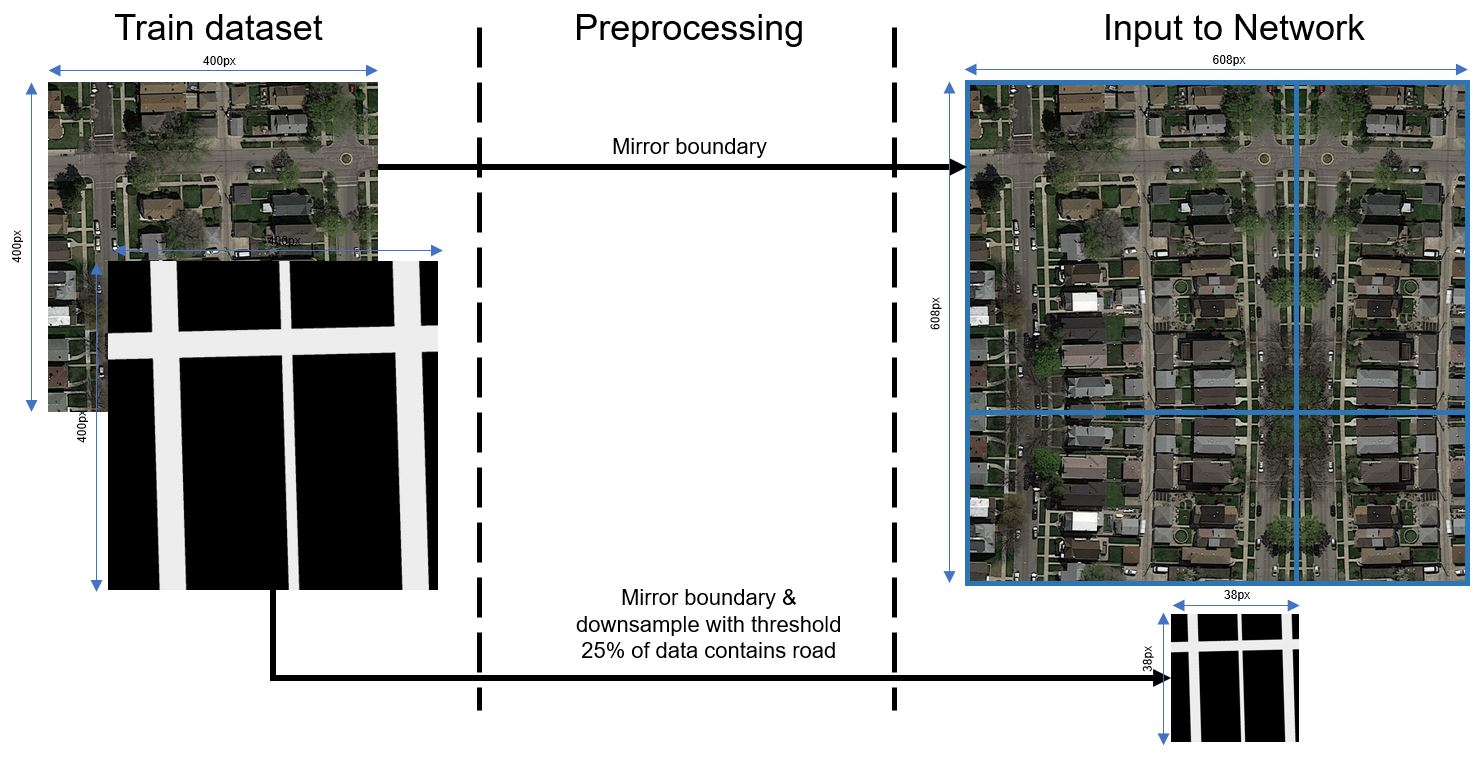
\includegraphics[width={8cm}]{preprocessing}
\caption{Preprocessing necessary for the training data. The given dataset (left) with dimensions 400x400 along with its pixelwise labelling are preprocessed (middle) using a mirror effect which enlarges the images to a resolution of 608x608 (right). Furthermore, the labels are downsampled to a 38x38 for each 16x16 image patch.}
\label{fig:preprocessing}
\end{figure}

\subsection{Image Augmentation}

To overcome the limitation of the small number of training samples, some data augmentation techniques have been used. The effectiveness of data augmentation was previously demonstrated \cite{Wang} for image classification. Because the roads of many of the provided training images are axis aligned it has been decided to implement data augmentation that compared to other previous approaches, arbitrarily rotates the images according to multiples of 90 degrees \cite{Pavllo2017}. The disadvantage of our approach is that the generation of these arbitrary rotations takes considerably more time. To maintain the advantage of the U-Net architecture about its fast training time \cite{Ronneberger2015}, the augmentation is split in two phases which are executed on different moments during the training. The first part of augmentation is only executed once every epoch, while the second part of it is applied to each training sample on each batch.

The first phase of augmentation includes steps such as randomly zooming (range 0.8-1.2), shearing (range 0 - 0.1), rotation (0 – 360) and height or width shifting (range 0 - 0.1) on the images. Finally, before generating each batch as input to the model, a rotation (by a 90 degree multiple) as well as a random mirroring are additionally applied. This second augmentation phase can be executed very fast during training time, while the first one needs more time. This technique allowed to overcome the disadvantages of the slow arbitrary rotation while still generating a higher number of different training samples.

\subsection{CNN Architecture}\label{architectures}

\begin{figure}
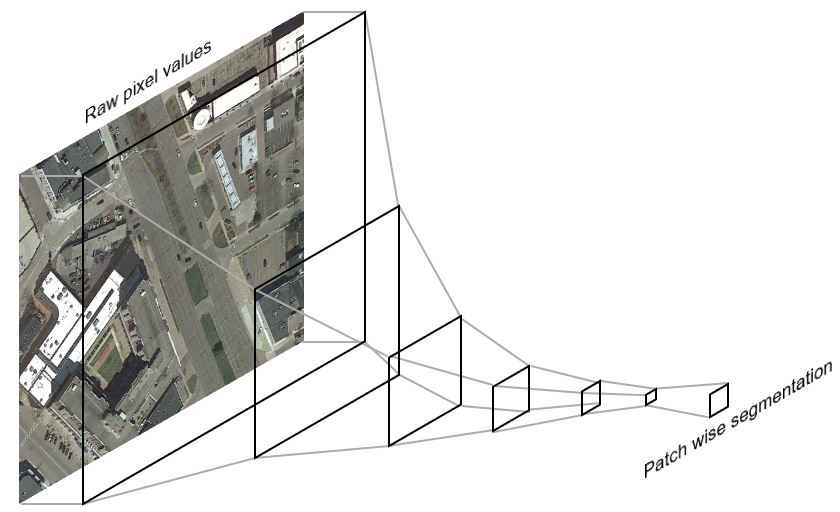
\includegraphics[width={8cm}]{network-visualisation}
\caption{Architecture of the proposed network. Visualizing the 7 layers used where the first 6 downsample the image and the 7th layer upsamples it again using a residual connection to layer 5 and outputs a patch wise segmentation.}
\label{fig:architecture}
\end{figure}

In order to achieve the desired pixel-to-patch prediction of the model, a truncated version of the U-Net \cite{Ronneberger2015}, as presented in table \ref{table:truncated_unet}, has been adopted. This architecture can be further visualized in figure \ref{fig:architecture}. The original implementation of the U-Net uses an up-sampling layer (e.g. layer 7) as many times as a down-sampling layer (e.g. layer 1 – 4) to output the same dimensions as the input. In this project this isn't desired, and the model has been truncated to fit the newer needs where the dimension 38x38 corresponds to the desired patch size ($16 \cdot 38 = 608$).

To further limit the arising of overfitting on the training data, a supplementary adapted version of regularization is proposed as shown in able \ref{table:truncated_regularized_unet}. The adaptions were inspired by \cite{Pavllo2017}. In particular, instead of using \textit{rectified linear units} (ReLU) as activation function, like it is proposed by the U-Net implementation \cite{Ronneberger2015}, \textit{Leaky ReLU} is used to avoid the \textit{dead filter effect} which some units can experience. \textit{Leaky ReLUs} are defined as $f(x) = \max(\alpha x, x)$. After different trials, it has been found empirically that the value $\alpha=0.1$ yields good results. This alpha setting is confirmed to be a good one also in other methods \cite{Pavllo2017}. Furthermore, in order to regularize the model, after each level a dropout layer is added with a rate of $0.25$. The output layer is penalized using a L2-regularizer.

\begin{table}[]
\centering
\begin{tabular}{lll}
\hline
Level & Layer                                                                       & Dimension  \\ \hline
0     & input                                                                       & 608x608x3  \\
1     & \begin{tabular}[c]{@{}l@{}}2 x conv(3x3, ReLU)\\ maxpool(2x2)\end{tabular}  & 304x304x32 \\
2     & \begin{tabular}[c]{@{}l@{}}2 x conv(3x3, ReLU)\\ maxpool(2x2)\end{tabular}  & 152x152x64 \\
3     & \begin{tabular}[c]{@{}l@{}}2 x conv(3x3, ReLU)\\ maxpool(2x2)\end{tabular}  & 76x76x128  \\
4     & \begin{tabular}[c]{@{}l@{}}2 x conv(3x3, ReLU)\\ maxpool(2x2)\end{tabular}  & 38x38x256  \\
5     & 2 x conv(3x3, ReLU)                                                         & 19x19x512  \\
6     & \begin{tabular}[c]{@{}l@{}}up-conv(2, 2)\\ 2 x conv(3x3, ReLU)\end{tabular} & 38x38x256  \\
7     & conv(1x1, Sigmoid)                                                          & 38x38x1    \\ \hline
\end{tabular}
\caption{U-Net, truncated for pixel to patch prediction.}
\label{table:truncated_unet}
\end{table}

\begin{table}[]
\centering
\begin{tabular}{lll}
\hline
Level & Layer                                                                       & Dimension  \\ \hline
0     & input                                                                       & 608x608x3  \\
1     & \begin{tabular}[c]{@{}l@{}}2 x conv(3x3, Leaky ReLU)\\ maxpool(2x2) \\ dropout(0.25) \end{tabular}  & 304x304x32 \\
2     & \begin{tabular}[c]{@{}l@{}}2 x conv(3x3, Leaky ReLU)\\ maxpool(2x2) \\ dropout(0.25) \end{tabular}  & 152x152x64 \\
3     & \begin{tabular}[c]{@{}l@{}}2 x conv(3x3, Leaky ReLU)\\ maxpool(2x2) \\ dropout(0.25) \end{tabular}  & 76x76x128  \\
4     & \begin{tabular}[c]{@{}l@{}}2 x conv(3x3, Leaky ReLU)\\ maxpool(2x2) \\ dropout(0.25) \end{tabular}  & 38x38x256  \\
5     & \begin{tabular}[c]{@{}l@{}}2 x conv(3x3, Leaky ReLU)  \\ dropout(0.25)               \end{tabular}  & 19x19x512  \\
6     & \begin{tabular}[c]{@{}l@{}}up-conv(2, 2)\\ 2 x conv(3x3, Leaky ReLU)                 \end{tabular}  & 38x38x256  \\
7     & \begin{tabular}[c]{@{}l@{}}conv(1x1, Sigmoid)\\ L2(10E-6)                                 \end{tabular}  & 38x38x1    \\ \hline
\end{tabular}
\caption{U-Net, truncated, dropout \& LeakyRelu for pixel to patch prediction.}
\label{table:truncated_regularized_unet}
\end{table}

\subsection{Loss function}

The final score on the Kaggle competition \cite{KaggleCompetition} is calculated using the F1-Score which was used for the training the model as well.

\section{Results}

Here the two proposed methods from section \ref{architectures} are compared with two baselines which have been chosen to be the all zero prediction and the CNN model advanced in \cite{Pavllo2017} which does patch-to-patch prediction. According to our knowledge, the latter was the highest performing architecture implementation for this problem. \\
The neural networks are all implemented using Keras with Tensorflow as backend. All the models are evaluated using a train/validation split of 2/3 of the training dataset.

The results are presented in table \ref{results-list}. The train and validation scores displayed are the one obtained at the end of the training. The test-score was found based on the results on the Kaggle competition \cite{KaggleCompetition}. For the CNN model proposed in \cite{Pavllo2017} and the all zero prediction there are no train and validation scores available. Based on the test set, it is possible to conclude that the proposed methods based on the re-adapted U-Net architecture outperform the patch-wise trained and predicting CNN model. Comparing the models presented in section \ref{architectures}, it turns out that the expected result for the additional regularization with dropout lead to a closer training/validation difference and finally to a better score on the test set.

Interesting is the fact that the all background baseline where each patch is predicted to be non-road obtains an already high test result.

An example of prediction using U-Net truncated with dropout \& Leaky Relu, which is the one performing best, is shown in figure \ref{fig:result}. The last submission to the Kaggle competition was trained with all the provided training data and no validation-set. The obtained score for the Kaggle competition is $0.90242$.

\begin{table}[]
\centering
\begin{tabular}{|l|l|l|l|}
\hline
\textbf{Model}                             & \textbf{Train} & \textbf{Val} & \textbf{Test} \\ \hline
All background & -                    & -                         & 0.85                \\ \hline
CNN \cite{Pavllo2017} & -                    & -                         & 0.87                \\ \hline
U-Net, truncated                           & 0.96                 & 0.85                      & 0.90                \\ \hline
U-Net, truncated, dropout     & 0.94                 & 0.86                      & 0.89                \\ \hline
\end{tabular}
\caption{Comparison of different methods where each column shows the scores obtained during training, validation and test.}
\label{results-list}
\end{table}

\begin{figure}
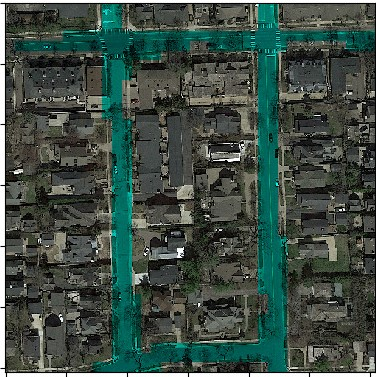
\includegraphics[width={8cm}]{result}
\caption{Example prediction using U-Net, truncated, dropout \& LeakyRelu where the predicted roads are marked as blue.}
\label{fig:result}
\end{figure}

\section{Discussion}

Even for a human it is not always possible to correctly classify a patch into road or non-road. This shows the difficulty of obtaining a perfect predictor for this task. Visually analazing the prediction in figure \ref{fig:result}, the predictions of the network closely resemble the expected result by a human. Examining the top horizontal street some road prediction discontinuities are evident. A proposal for additional work could be to either find a way to penalize discontinuities or, alternatively, correct them in a post-processing step.

To further improve the result we propose to train the model on more data. In \cite{Kaiser2017} it was shown that training on datesets from other data sources of aerial images can improve the prediction. Additional training data for this task is indeed available (e.g. Google Maps, OpenStreetMap). Therefore, additional work could be done in obtaining and preprocessing the new data in order to be advantageous for better predictions on test.

\section{Summary}

We proposed an image-to-patch prediction using the U-Net architecture which is based on a CNN model. This enabled us to predict if a given patch of an aerial image is occupied by a certain threshold area of road or not. To permit the U-Net architecture to predict on images-to-patches it was necessary to truncate the end of the original network architecture and to directly predict to the 38x38 output labels. The final proposed model adds dropout layers to counteract overfitting. Some attempts to overcome the problem of a small training dataset by using image augmentation were performed. A comparison of our method to the two baselines suggests that the proposed model surpasses them.




\bibliographystyle{IEEEtran}
\bibliography{bibliography}
\end{document}
